\documentclass[12pt]{article}
\usepackage[margin=2cm]{geometry}
\usepackage{graphicx}
\usepackage{mathtools}
\usepackage{svg}
\usepackage{enumitem}
\usepackage{float}
\newcommand{\defeq}{\vcentcolon=}

\usepackage[pagebackref]{hyperref}
\hypersetup{
    colorlinks,
    linkcolor={red!95!black},
    citecolor={blue!100!black},
    urlcolor={violet!100!black}
}

\title{Problem 9: Water Laser \\ Theory Document}
\author{William Dracopoulos}
\date{\today}

\begin{document}

\maketitle

\section{Problem statement}\label{sec:problem}

A shallow water tank mechanically excited by a motor features some of the basic ingredients of a laser (i.e. a cavity and an amplifier). To what extent can this simple analogy capture more complex aspects of laser physics, such as spontaneous and stimulated emission, population inversion, Q switching, and others?

\section{Basics of (the inside of) a laser}\label{sec:basics}

Stimulated emission is the most important part of the functioning of a laser. Imagine a stable, free-floating atom. If a free electron collides with it, it might knock one of the electrons in the atom into a higher energy level. Call the energy gained between states $\Delta E$ This electron will eventually come back down as it was before, to its "ground state". In doing this, if it has nowhere else to release this energy, the electron will create a photon which flies away from the atom with exactly $h\nu = \Delta E$, so that energy can be conserved.

This will eventually happen naturally, but a much quicker way for it to happen is if a new photon with $h\nu = \Delta E$ flies in and collides with the excited electron. The electron will then fall back to the ground state, and we will be left with two photons with energy $\Delta E$. It is characteristic of lasers that all of the light they emit has the same wavelength and is in phase. This is because the ejected photon has the same energy and phase as the one which stimulates it.

The goal is to get a large number of atoms to be excited to the same $\Delta E$, then wait for a spontaneous emission to start a chain reaction of stimulated emissions, where each photon collision creates one more photon. To keep the chain reaction going, photons should be kept bouncing around within the system, and electrons within the atoms must be constantly excited so that more photons can be produced after the first collisions.

An atom with an electron in an energy level higher than ground state will be called an "excited atom". Otherwise, it will be called a "ground-state atom." Typically, each atom will have a maximum of of one electron in a higher energy state. When there are more atoms in an excited state than in the ground state, it's called "population inversion," and its what allows lasers to create light.

\vspace{0.5cm}

\noindent Figure \ref{fig:cavity_diagram} features a simple diagram of a laser cavity and amplifier, the inside of a laser. The atoms of the gain medium are usually electrically excited (free electrons are collided into the atoms' electrons) so that stimulated emission can occur. This process is called "pumping". The medium can be solid, liquid, or gas, as long as it is conducive to stimulated emission.

In the simplified model shown in Figure \ref{fig:cavity_diagram}, the amplifier can be thought of as simply the gain medium and the device which electrically excites it, while the cavity can be thought of as the space around it, including the reflectors.

An important design consideration of the cavity is its length. It is made so that a standing wave of wavelength $\lambda = \frac{c}{\nu} = \frac{h\,c}{\Delta E}$ can exist within it. This ensures that only the desired wavelength of light exists within the laser, as other wavelengths will interfere with themselves while reflecting.

\begin{figure}[H]
    \centering
    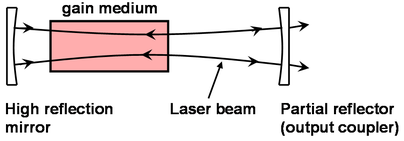
\includegraphics{figures/cavity.PNG}
    \caption{Basic setup of the inside of a laser.}
    \label{fig:cavity_diagram}
\end{figure}

The amplifier is made so that all photons leave the gain medium going either "forward" or "backward" as seen in Figure \ref{fig:cavity_diagram}. To keep the chain reaction going, there are mirrors on both ends to reflect all of the photons back into the gain medium for a new round of stimulated emission. However, since the goal of a laser is to get light \b{out} of the device, the front mirror lets some light through. This is the light we see as the laser beam.

\vspace{0.5cm}

\noindent The only other concept mentioned in the problem statement is Q switching.

Imagine opening one end of the laser. Any photons that are created will simply leave. This gives the amplifier a chance to excite the electrons of almost all of the atoms without getting knocked back to ground state, as no chain reaction is happening. Then, when the end is closed again, the chain reaction will restart. Since almost all of the atoms are excited, the chain reaction will begin really strongly and a high-intensity burst of light will come out of the laser.

This effect will quickly die down however, as all of the excited electrons will get knocked back down to ground state quickly. The laser will then continue operating with only as much intensity as permitted by the pumping rate.



\section{Setup/Approximations}\label{sec:setup}

The picture of particles bumping to each other and producing photons out of nothing is convenient and easy to understand, but not possible to use for this project. "A shallow water tank mechanically excited by a motor" mentioned in the problem statement seems to imply that the action is going to be happening in the waves of the water, mimicking waves in the electric field (ie, light), with the motors being the source of interaction with the field. The motor should therefore mimic the atoms.

The water surface is certainly only two-dimensional, with the height of the waves representing one dimension of field values. In other words, a wavy water surface can be represented as a field $h(x, y)$. This can mimic a two-dimensional electric field where all light waves are vertically polarized. Imagine a still tank of water, with a plane at the water level. Add a small ripple to the water, then draw a vertical vector from the plane to the new rippled water height. That vector can represent a vertical vector in the analogous two-dimensional electric field.

Section \ref{sec:electric-water} will describe how the water acts and how it's different to the electric field. Section \ref{sec:motor-atom} will begin to explain how to create an analogue to atoms in the tank, and how they will interact with the waves.



\section{Characterizing Water Waves}\label{sec:electric-water}

\b{In the limit of small waves and shallow water} (water depth less than a wavelength), motion of the water in the tank can be described by the Shallow Water Equations. If the waves are too large splashing might occur, and if the water is too deep undercurrents and more complex water movement will occur. By staying within this approximation, the water tank will look most like the electric field.

The following are some of its parameters:

\begin{itemize}[itemsep=0em]
    \item $H$: average water level (where the tank is filled to)
    \item $h$: wave height (the real water height is h+H)
    \item $u$: horizontal water velocity in the x-direction
    \item $v$: horizontal water velocity in the y-direction
    \item $g$: acceleration due to gravity
    \item $\nu$: the kinematic viscosity of water
    \item $\rho$: water's density
    \item $k$: the viscous drag coefficient
    \item $P_{ext}$: external pressure applied to the water surface
\end{itemize}

And here are the equations:

\begin{equation}\label{eqn:swe_h}
    \frac{\partial h}{\partial t} + \frac{\partial (H + h) u}{\partial x} + \frac{\partial (H + h) y}{\partial y} = 0
\end{equation}

\begin{equation}\label{eqn:swe_u}
    \frac{\partial u}{\partial t} + u \frac{\partial u}{\partial x} + v \frac{\partial u}{\partial y} + g \frac{\partial h}{\partial x} + ku + \frac{1}{\rho} \frac{\partial P_{ext}}{\partial x} = \nu \left( \frac{\partial^2 u}{\partial x^2} + \frac{\partial^2 v}{\partial y^2} \right)
\end{equation}

\begin{equation}\label{eqn:swe_v}
    \frac{\partial v}{\partial t} + u \frac{\partial v}{\partial x} + v \frac{\partial v}{\partial y} + g \frac{\partial h}{\partial y} + kv + \frac{1}{\rho} \frac{\partial P_{ext}}{\partial x} = \nu \left( \frac{\partial^2 u}{\partial x^2} + \frac{\partial^2 v}{\partial y^2} \right)
\end{equation}

Note: $P_{ext}$ is the only term which drives the water's motion. Additionally, $\nu$ is very small relative to the other terms, $\rho \approx 1000 \frac{kg}{m^3}$, and $k \approx 1$.

\vspace{0.5cm}

\noindent If this was written as a wave equation like that of the electric field, it would instead take the form

\begin{equation}
    \frac{\partial^2 h}{\partial t^2} = v^2 \left( \frac{\partial^2 h}{\partial x^2} + \frac{\partial^2 h}{\partial y^2} \right)
\end{equation}

Where $v$ is some constant speed at which all waves travel.

\vspace{0.5cm}

\noindent An important consideration from the Shallow Water Equations is that the waves travel at different speeds depending on their amplitude, $v \approx \sqrt{g\,|H+h|}$. This alone makes it impossible to create a complete analogy to the electric field in water.

Additionally, waves will slow down and lose amplitude due to the drag and viscosity terms. This means that the wavelengths of waves in the water will increase and eventually the waves will die out as they travel.

\section{Making a Motor Act Like an Atom}\label{sec:motor-atom}

A motor will be placed in the water tank to produce waves within the water, along with a sensor to detect the water height near the motor. This will allow it to simulate an atom which reacts to the electric field around it, and also interacts with the field by putting waves into it.

Practically, the motor might be made into a fan which is just above the water, applying a pressure to the water surface. This would correspond directly to the $P_{\text{ext}}$ term in the Shallow Water Equations \ref{eqn:swe_u} and \ref{eqn:swe_v}. Pushing the water surface downwards this way will be easy, but pulling upward would require way more power from the fan. Instead, a baseline pressure can always be applied by the fans, in which case pushing down would mean the fan blows harder, and pulling up means slowing the fan so that the water lifts back up to its normal level.

The sensor can be implemented by dying the water so that it absorbs light going through it, placing a light under the tank, and using a photodiode at the top of the tank to detect how much light got through. The amount of light coming through can be correlated to the height of the water using the Beer-Lambert law.

It is unclear whether these two devices will have enough precision and speed to do what is required in terms of detecting and generating quick-moving waves.

In reality, a single motor will represent a cluster of atoms, for reasons explained in Section \ref{sec:lorentz-laser}. However, multiple motors corresponding to multiple distinct clusters can be used to show not only how atoms interact with the waves, but also how they interact with each other via the waves.

To decide exactly how this simulated atom will interact with the water around it, a model of atom-light interaction must be decided, taking into account the physical limitations of doing this with water and motors.

Note that all of the atoms' behaviour (pumping, oscillation, excitement, etc.) would be simulated within electronics and the only physical thing going on in the tank is the beginning and the end of the process: reading the water height and applying pressure to the water surface.

\section{Model of Atom-Light Interactions}\label{sec:atom-light}

The best quantum-mechanical description of how light waves (as opposed to the simplified particle view described in Section \ref{sec:basics}) interact with atoms are the Maxwell-Block equations. However, they use their own set of assumptions and use the electric field values in the form of complex numbers, which is completely impossible to measure for a real water. For this section, only real electron and the real electric field will be discussed. How this maps to the motors and water will be dealt with later.

Another option is the classical Lorentz Oscillator Model. It is much simpler and easier to build off of. This will be simplified to only up-down polarization for the reason explained in Section \ref{sec:setup}. It goes like so:

Imagine an electron as a small mass bound to a stationary atom by a spring-like force. This electron will have some damping on its motion corresponding to losing energy through the emission of waves in the electric field. Since it is a charged particle, it will also get pushed by the electromagnetic force, represented by the electric field around it. Its equation of motion is the following:

\begin{eqnarray}
    F_{\text{damping}} + F_{\text{spring}} + F_{\text{driving}} = m \frac{d^2 r}{dt^2}
    \\
    \frac{-m}{\tau}\frac{dr}{dt} - kr - e E = m \frac{d^2 r}{dt^2}
\end{eqnarray}

\begin{equation}\label{eqn:r-motion}
    \frac{d^2 r}{dt^2} + \frac{1}{\tau} \frac{dr}{dt} + \frac{k}{m} r = \frac{-e}{m}E
\end{equation}

Where $E$ is the electric field (remember, all vectors are only pointing in the up-down direction), $r$ is the displacement of the electron from the center of the atom (again, only in the up-down direction), $m$ and $-e$ and the mass and charge of the electron respectively, $\tau$ is the "relaxation time," related to how quickly the electron loses energy, and $k$ is the strength of the force keeping the electron to the atom.

$r$ is then related to the "polarization" of the electron,

\begin{equation}\label{eqn:polarization}
    p = -e r
\end{equation}

And finally, this polarization drives the motion of the electric field, as seen in Maxwell's equations.

\begin{equation}\label{eqn:maxwells}
    \nabla^2 E - \frac{1}{c^2} \frac{d^2 E}{d t^2} = \frac{1}{\epsilon_0 c^2} \frac{d^2 p}{dt^2}
\end{equation}

Note that $p$ will be zero everywhere other than directly under an electron. So an accelerating electron drives the electric field under in, then that bump gets carried away by the electric field as a wave\footnote{This is why the motor in the water tank only needs to push and pull at the water directly under it.}.

\subsection{The Impact of Constant $k$}

As with any damped driven harmonic oscillator like this electron, the natural frequency is defined by $\omega_0 = \sqrt{\frac{k}{m}}$. This represents approximately the frequency of the driving force which interacts most strongly with the oscillator. In this case, with sufficiently weak damping, any light within the laser cavity which isn't of frequency $\omega_0$ will effectively be ignored by the atoms and will eventually die out.

This means that all light in the cavity and all light coming out of the cavity will have the same frequency $\omega_0$. This aligns with lasers producing only a single frequency of light.

\subsection{Lasers in the Lorentz Model}\label{sec:lorentz-laser}

Despite being a good foundation, the Lorentz model is not enough to explain anything which is unique to lasers. To do this, some inspiration must be taken from the Maxwell-Bloch Equations.

To get spontaneous and stimulated emission, population inversion, and Q switching, the electrons need to have the excited state - ground-state behaviour. First, an equation describing the number of excited and ground-state atoms needs to be derived. The following is based on the same logic as used in the Maxwell-Bloch equations:

\vspace{0.5cm}

\noindent Imagine a cluster of atoms. The fraction of excited atoms will be denoted $n_E$ and the fraction of ground-state atoms will be denoted $n_G$.

Let $R$ be the pumping rate per atom, now quickly each ground-state atom is expected to be electrically excited by the pumping system.

Atoms which are already excited have a tendency to naturally lose energy and go back to the ground state. Let the average time it takes for this to happen spontaneously be denoted by $T$, the "relaxation time".

Finally, a wave of light passing through an excited atom tends to make it drop to the ground state at a rate proportional to the intensity of the wave $I$. Let the proportionality constant be $\alpha$. Additionally, a wave of light passing through a ground-state atom tends to excite the atom at the same rate proportional to $I$.

If there enough atoms in the cluster, $n_E$ and $n_G$ can be thought of as approximately continuous variables and therefore a derivative can be taken. Therefore the above paragraphs can be translated into a differential equation.

\begin{equation}\label{eqn:excitement-diff}
    \frac{d\,n_E}{dt} = R - \frac{n_E}{T} - \alpha I n_E + \alpha I n_G
\end{equation}

Letting $n = n_E - n_G$ (the "net excitement") and $n_T = n_E + n_G = 1$, Equation \ref{eqn:excitement-diff} becomes

\begin{equation}\label{eqn:net-excitement}
    \frac{dn}{dt} + \left(\frac{1}{T} + 2 \alpha I \right) n = 2R - \frac{1}{T}
\end{equation}

\vspace{0.5cm}

\noindent To get a sense of how this equation acts, $I$ can be assumed to be constant and $n$ can be solved as a function of time $t$. The initial net excitement will be called $n_0$.

\begin{equation}
    n(t) = \left(n_0 - \frac{2R - \frac{1}{T}}{\frac{1}{T} + 2 \alpha I}\right)e^{-\left(\frac{1}{T} + 2 \alpha I\right)t} + \frac{2R - \frac{1}{T}}{\frac{1}{T} + 2 \alpha I}
\end{equation}

As $t \rightarrow \infty$, $n \rightarrow \frac{2R - \frac{1}{T}}{\frac{1}{T} + 2 \alpha I}$, showing that the system comes to some kind of equilibrium according to those parameters. This is what is expected, since after a short amount of time, real lasers do reach equilibrium and produce a steady beam.

As long as $2R > \frac{1}{T}$, the laser will come to equilibrium with $n > 0$. In other words, more atoms will be excited than ground-state. This means that population inversion will be reached, and the gain medium will produce more light than it absorbs.

Additionally, once population inversion is reached it will never be lost until pumping is turned off. This is because no matter the value of $I (> 0)$, the sign of the equilibrium position will always be positive.

The value of $I > 0$ and $n > 0$ at equilibrium will be set to whatever is needed to compensate for the energy lost (mostly due to the front mirror being only partially reflective to produce a laser beam as seen in Figure \ref{fig:cavity_diagram}).

\subsubsection{Calculating the Intensity $I$ In a Water Wave}

Equation \ref{eqn:net-excitement} requires the wave intensity $I$ to be known at the position of the atom. Since waves in water are fundamentally different from those in the electric field, an equation for $I$ must be derived separately.

Intensity is defined as the energy density of the wave within a volume multiplied by the speed of the wave through that volume

\begin{equation}
    I = \frac{dE}{dV} ||\mathbf{w}||
\end{equation}

Where $\frac{dE}{dV}$ is the energy density and $\mathbf{w} \defeq (u, v)$ as defined in the Shallow Water Equations \ref{eqn:swe_h}, \ref{eqn:swe_u}, and \ref{eqn:swe_v}. $||\mathbf{w}||$ therefore represents the wave speed. Note that $u = u(x, y, t)$ and $v = v(x, y, t)$, both are functions of time and space. Because of the shallow water approximation, the water assumed not to be moving in the $z$ direction, only horizontally.

Calculating $dE$ for a position (x, y, z) within the water tank,

\begin{eqnarray}
    dE = dE_K + dE_P
    \\
    dE_K = \frac{1}{2}\,dm\,\mathbf{w}^2
    \\
    dE_P = dm\,g\,z
\end{eqnarray}

Since the density of water $\rho$ is known, $dm = \rho\,dV$ can be used

\begin{eqnarray}
    dE = \frac{1}{2}\,\rho\,dV\,\mathbf{w}^2 + \rho\,dV\,g\,z
    \\
    I = \frac{\frac{1}{2}\,\rho\,dV\,\mathbf{w}^2 + \rho\,dV\,g\,z}{dV}||\mathbf{w}||
\end{eqnarray}

As with the Shallow Water Equations, each vertical column of water will be treated as a single element with uniform momentum. In other words, the equations are integrated across the $z$ direction. Similarly, each vertical column will be treated as a single element with uniform energy by integrating across $z$, from $0$ to the water height $h + H$ (from Equation \ref{eqn:swe_h}). Instead of each point in the 3D space of the water tank having its own intensity, simply each vertical column of water will have its own intensity. Expanding $dV$ with $dV = dx\,dy\,dz$:

\begin{equation}
    I = \frac{\frac{1}{2}\,\rho\,dx\,dy\,dz\,\mathbf{w}^2 + \rho\,dx\,dy\,dz\,g\,z}{dx\,dy\,dz} ||\mathbf{w}||
\end{equation}

\begin{equation}
    I = \frac{\frac{1}{2}\,\rho\,dz\,\mathbf{w}^2 + \rho\,dz\,g\,z}{dz} ||\mathbf{w}||
\end{equation}

\begin{equation}
    I \approx \frac{\int_{z=0}^{z=h+H} \left[ \frac{1}{2}\,\rho\,dz\,\mathbf{w}^2 + \rho\,dz\,g\,z \right] }{\int_{z=0}^{z=h+H} dz} ||\mathbf{w}||
\end{equation}

\begin{equation}
    I \approx \frac{\frac{1}{2}\,\rho\,(h+H)\,\mathbf{w}^2 + \frac{1}{2}\rho\,(h+H)^2\,g }{h+H} ||\mathbf{w}||
\end{equation}

\begin{equation}
    I \approx \frac{1}{2}\,\rho\,||\mathbf{w}||^3 + \frac{1}{2}\rho\,(h+H)\,g\,||\mathbf{w}||
\end{equation}

\subsection{How the Atom Clusters use $n$}

As mentioned, this classical Lorentz Model is inconsistent with the idea of atom excitement. There is no physically accurate place to use $n$ within the model, so it will seem arbitrary but it will produce a result looking like what quantum mechanics expects. Here is the logic:

Imagine a stationary electron around its atom, with a wave coming through the electric field which looks like a sine wave, starting at 0 and increasing. Look at Equation \ref{eqn:r-motion}, just as the wave hits the electron, $E > 0$ so $\frac{d^2r}{dt^2} < 0$. Therefore by Equation \ref{eqn:polarization} $\frac{d^2p}{dt^2} > 0$, and by Equation \ref{eqn:maxwells} $\frac{d^2E}{dt^2} < 0$. The electric field is therefore accelerated in the opposite direction to its position because of the presence of the atom. This has the effect of a ground state atom absorbing light.

Now imagine the same situation but with $p = er$, a flipped sign. Then $\frac{d^2E}{dt^2} > 0$ instead, and the electric field will be accelerated in a way which amplifies the wave.

With the fraction $n_E$ of atoms being excited and $n_G$ being ground-state, summing up the polarization of the entire clump of atoms yields

\begin{eqnarray}
    n_E\,e\,r -n_G\,e\,r = p
    \\
    n\,e\,r = p
\end{eqnarray}

The model for atom-light interactions is now complete.

\section{Design Considerations of the Water Tank}\label{sec:tank-design}

The water tank must be created to be similar to a laser cavity as described in Section \ref{sec:basics}.

First, the cavity should be designed at a length so that standing waves can be supported at the wavelength of the laser's light. This ensures minimal destructive interference within the cavity.

The back mirror can simply be a solid for the water waves to bounce off of it. The front and back mirrors could be curved like in Figure \ref{fig:cavity_diagram} to force the wave toward the center of the cavity where the gain medium is.The front mirror needs to let some of the wave through. A way to do this might be to make a deep groove in the bottom of the tank. Since the speed of the wave is $\approx \sqrt{g |h+H|}$, increasing $H$ by making the tank deeper along some part will have same same effect of increasing the index of refraction in the electric field. Therefore that part of the tank will act as a material like glass, causing some reflection and some transmission. If that is impossible to do practically, the front reflector could instead be a solid wall with slits cut into it to let some of the wave through.

The other wall of the tank could just be solid and let the wave totally reflect off of them (instead of having a system to drive the waves away from them and toward the front and back walls like in real lasers).

The gain medium will sit in the center of the cavity and consist of at least one atom cluster (at least one motor).

Outside of the cavity, the water tank can be extended so that the laser beam can be viewed propagating through empty space. To showcase the absorbing properties of the atom clusters, at the end of the beam can be some atom clusters which are not being pumped (start off in ground state). The beam should mostly disappear as it reaches those atoms, like how a laser pointer becomes less visible when shining it on a black surface.

\end{document}